\section{Analyse und Bewertung der Teilprozesse und Stakeholder}

In diesem Kapitel werden die Stakeholder des neu zu entwickelnden Systems für die Anrechnung von Studien – und Prüfungsleistungen behandelt. Dabei wird auf deren Rolle im bisherigen Prozess eingegangen und die Veränderungen durch eine mögliche Einführung eines neuen Systems beschrieben. Das neue System hat vier Stakeholder: die Mitarbeiter des Prüfungsamtes, die Mitglieder des Prüfungsausschusses, die Studierenden und die zuständige IT-Abteilung.

\resizebox{\textwidth}{!}{%
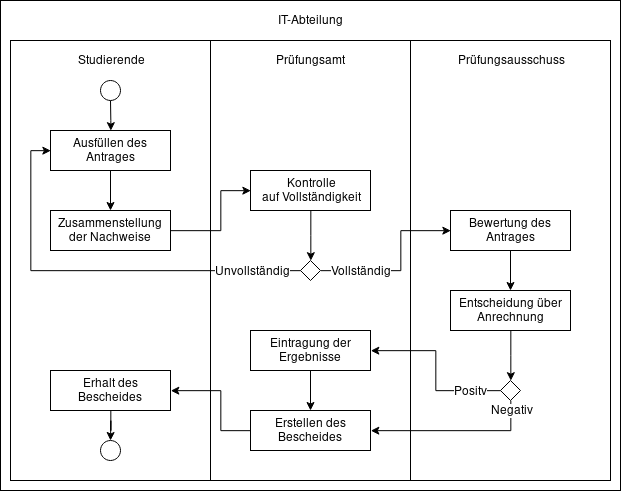
\includegraphics{../../images/analoger_prozess.png}%
}

\subsection{Prüfungsamt}

Im bisherigen Prozess nehmen die Mitarbeiter des Prüfungsamts die Anträge der Studierenden entgegen und bereiten die Dokumente für die Weitergabe an den Prüfungsausschuss vor. Nach der Überprüfung der Dokumente auf Vollständigkeit werden die Anträge an den Prüfungsausschuss weitergegeben. Wenn der Ausschuss seine Entscheidung über die Anrechnung getroffen hat, nimmt das Prüfungsamt das Ergebnis entgegen und trägt etwaige Noten in das Notenverwaltungssystem ein. Den Studierenden wird anschließend Bescheid über die Entscheidung des Ausschusses gegeben.

\subsection{Prüfungsausschuss}

Momentan nehmen die Mitglieder des Prüfungsausschusses die zentrale Rolle in der Anrechnung von Studien – und Prüfungsleistungen ein. Der Prüfungsausschuss erhält die Anträge und Dokumente der Studierenden in aufbereiteter Form vom Prüfungsamt. Danach entscheidet der Ausschuss darüber, ob die Anrechnung ganz, teilweise oder gar nicht vorgenommen wird. Das Ergebnis der Entscheidung wird dann an das Prüfungsamt zurückgegeben.

\subsection{Studierende}

Die Hauptaufgabe der Studierenden ist es die, für die Anrechnung nötigen, Dokumente zu sammeln. Dazu gehören beispielsweise eine Beschreibung der Module und die Nachweise über die erhaltenen Noten. Die Anträge können dann im Moment auf zwei Wegen erstellt werden. Entweder füllen die Studierenden die vom Prüfungsamt bereitgestellten PDF-Vorlagen von Hand oder mit einem entsprechenden PDF-Reader aus oder sie benutzen einen bereits existierenden Assistenten, welcher nach Eingabe der Daten die PDFs automatisch ausfüllt. Nach dem Ausfüllen müssen die Anträge beim Prüfungsamt persönlich abgegeben werden. Die Möglichkeit einer Einreichung per Mail oder Online gibt es momentan nicht. Nach dem Entscheidungsprozess erfahren die Studierenden das Ergebnis per Mail und finden die dazugehörigen Noten im Notenverwaltungssystem.

\subsection{IT-Abteilung}

Aktuell hat die IT-Abteilung fast keinen Kontakt zum Anrechnungsprozess, sie pflegt lediglich die Funktionalität des E-Mail Servers und des bisherigen Notenverwaltungssystems.

\subsection{Studienfachberatung}

Die Studienfachberatung nimmt als Stakeholder eine spezielle Rolle ein, die nur indirekt am Anrechnungsprozess beteiligt ist. Zum einen kann sie zu Beginn als beratende Instanz zur Verfügung stehen, die den Prozess durch die Beratung des Studierenden einleitet. 
Im Verlauf der Anrechnung dient sie weiterhin als Ansprechpartner und Koordinator.

